\documentclass[11pt, titlepage]{article}
\usepackage{beamerarticle}
\usepackage[utf8]{inputenc}
\usepackage{amssymb,amsmath}

% Page settings
\usepackage[letterpaper, margin=1in]{geometry}
\usepackage{times} % palatino, lmodern
\usepackage{setspace}
\doublespacing
%\doublespacing  % \singlespacing 

% Appendix
\usepackage{appendix}

% Line numbers
%\usepackage{lineno}
%\linenumbers

% Links
\usepackage{hyperref}
\hypersetup{%
  colorlinks=false,% hyperlinks will be black
  linkbordercolor=red,% hyperlink borders will be red
  pdfborderstyle={/S/U/W 1}% border style will be underline of width 1pt
}

% Tables
\usepackage{array,booktabs,longtable,rotating}

% Position tables {here, top, bottom, page}
\makeatletter
\def\fps@table{htbp}
\makeatother

%% ... at the end of paper
\usepackage{endfloat}

% Graphics
\usepackage{graphicx,grffile}
\makeatletter
\def\maxwidth{\ifdim\Gin@nat@width>\linewidth\linewidth\else\Gin@nat@width\fi}
\def\maxheight{\ifdim\Gin@nat@height>\textheight\textheight\else\Gin@nat@height\fi}
\makeatother
% Scale images if necessary, so that they will not overflow the page
% margins by default, and it is still possible to overwrite the defaults
% using explicit options in \includegraphics[width, height, ...]{}
\setkeys{Gin}{width=\maxwidth,height=\maxheight,keepaspectratio}
% set default figure placement to htbp
\makeatletter
\def\fps@figure{htbp}
\makeatother



\setlength{\emergencystretch}{3em}  % prevent overfull lines
\providecommand{\tightlist}{%
  \setlength{\itemsep}{0pt}\setlength{\parskip}{0pt}}


%\usepackage{xcolor}
%\usepackage{framed}
%\colorlet{shadecolor}{orange!15}
\usepackage{floatrow}
\floatsetup[table]{capposition=top}
\floatsetup[figure]{capposition=bottom}

% Math environments
\newtheorem{proposition}{Proposition}
\newtheorem{define}{Definition}


% Thresholds, limits, bounds, etc.
\newcommand\deadline{\bar{t}}
\newcommand\target{\underline{y}}

% Competitions
\newcommand\race{\text{race}}
\newcommand\tournament{\text{tour}}

% Cost functions
\newcommand\ctime{c_{\tau}}
\newcommand\cscore{c_{y}}
\newcommand\cability{c_{a}}
\newcommand\costs{\cability(a_i)\cscore(y_i)\ctime(t_i)}

% Distribution of types
\newcommand\ability{a_i}
\newcommand\marginaltype{\hat{a}}
\newcommand\mtype{\hat{a}}
\newcommand\lotype{\underline{a}}
\newcommand\hitype{\bar{a}}



% Derivatives
\newcommand\dystar{\frac{\partial y^*(x,\target)}{\partial\target}dF_{N:N}(x)}

\title{Races or Tournaments? Theory and Evidence from the Field\thanks{Blasco: Harvard Institute for Quantitative Social Science, Harvard
University, 1737 Cambridge Street, Cambridge, MA 02138 (email:
\href{mailto:ablasco@fas.harvard.edu}{\nolinkurl{ablasco@fas.harvard.edu}}).}}
\providecommand{\subtitle}[1]{}
\subtitle{{[}PRELIMINARY AND INCOMPLETE{]}}
\author{Andrea Blasco \and Kevin J. Boudreau \and Karim R. Lakhani \and Michael Menietti}
\date{Last updated: 20 June, 2017}

\begin{document}
\maketitle
\begin{abstract}
We examine the performance of two different choices of contest design:
the race (where the winner is the first to achieve a minimum quality)
and the tournament (where the winner is the one with the highest quality
in a given period). After characterizing the optimal design, we report
results of a field experiment conducted to compare the performance of
three alternatives motivated by theory: the race, the tournament, and
the tournament with a minimum quality requirement. Outcomes in a race
are of comparable quality, supplied faster, and with lower participation
rates. Based on these findings, we show the optimal design under several
counterfactual situations.

\smallskip\noindent 
JEL Classification: M15; M52; O31.

\smallskip\noindent 
Keywords: races; tournaments; contest theory; crowdsourcing; innovation.
\end{abstract}


\clearpage

\section{Introduction}\label{introduction}

Contests have had and continue to have tremendous impact on economic
growth. Historically, awards offered by government agencies have
accelerated agricoltural innovation;\footnote{See ({\textbf{???}}) for a
  study on the impact of the awards offered by the Royal Agricultural
  Society on agricultural innovation in England at the beginning of 20th
  century.} lead to important improvements to navigation and
cartography;\footnote{See ({\textbf{???}}) for the history of the
  Longitude Prize and its impact of the winning solution on navigation.}
and contributed to the developmenet of the modern aviation
sector;\footnote{See ({\textbf{???}}) for the Orteig Prize.} among other
things. Today, contests have become even more significant as a
mainstream managment tool, not limited to government agencies, but also
including philantropic organizations and private firms that recur
repeatedly to contests for numerous purposes: from promoting in-house
R\&D efforts (xxxx) to reaching out to online communities of freelancers
for crowdsourcing internal functions (marketing, data analysis, software
production).

While the economic relevance of contests is well recognized (xxxx), the
issue of the optimal design is still wide open. In this paper, we
address this issue by comparing two different choices of design
regarding the competition style of the contest. One is the ``race''
competition, where prizes are offered to the competitor that first
reaches a fixed performance target. The other is the ``tournament''
competition, where prizes are offered to the competitor that does best
relative to others by a given deadline. Familiar examples of races are
the Longitude rewards offered by the British government in 1714, the
Orteig Prize in 1919, and, more recently, the Netflix prize in 2009;
while most architectural competitions, the Golden Carrot Contest in
1992, the Defense Advanced Research Project Agency (DARPA) series of
Grand Challenges between 2004 and 2013, and the Progressive Insurance
Automotive X-Prize in 2010 are all examples of tournaments.\footnote{See
  Wikipedia article on ``Inducement prize contest''
  (\url{https://en.wikipedia.org/wiki/Inducement_prize_contest}) for a
  list of these contests with links to their descriptions. The Golden
  Carrot Contest has been described by Taylor (1995).}

Races and tournaments are very general forms of competition. And an
extensive literature exists that has focused on races, in the context of
patent races, and tournaments separetely. With only a few papers in
economics comparing race and tournament in a single framework. A
underxxxx that is perhaps becayse in many situations the choice seem
imposed by the environment (as in the case of the legal environment
defining a patent race) rather than a straightforward choice of contest
design. In addition, and from a contest design perspective, the choice
between race and tournament competitions is difficult to examine: xxxx.
A natural way to examine the issue is via modeling choices as a function
of the contest sponsors's preferences towards two desirable, but often
incompatible, goals: \(i\)) maximizing revenues through raising the
efforts of competitors while \(ii\)) lowering the time it takes to
complete a given job. It is unclear, however, how either two competition
formats will solve this trade-off. On the one hand, a fixed deadline may
accelerate production in tournaments. On the other, a too short deadline
may deter entry, thereby lowering revenues from competitors effort.
Likewise, a time competition may encourage competitors to reach a given
target faster, but it may also limit competition if the target can be
reached only by a few competitors. Alternatively, the choice between
tournaments and races can be seen as the response to ``efficiency''
concerns of the contest sponsors. Under this view, races and tournaments
may lead to the same expected outcomes in terms of time or effort but
lead to different duplication costs by regulating ``entry'' into the
contest {[}as discussed by Fullerton Mcafee, xxxx{]}. Hence, the ``time
preferences'' story and the ``efficiency'' are two possible explanation
for using a race or a contest.

In this article, we investigate the choice between races and tournaments
both theoretically, and empirically in the field. We proceed in two
ways. First, we develop a contest model that encompasses both the race
and the tournament in a single framework. Exploring the duality of the
model, we compare equilibrium behaviors under both competitive formats
and characterize the optimal choice for the contest designer. Then, we
design and execute an experiment to test the implications of the theory
in the field, and xxxx providing policy recommendations.

Our theoritical approach extends the contest model introduced by
Moldovanu and Sela (2001) to a situation in which xxx decide both time
and quality. Thus, contests have an all-pay structure by which
participants pay an immediate cost for an uncertain future reward. The
decision of timing and quality is made under the uncertainty of the
costs of the rivals. The contest designer wants to maximize reveues and
has preferences for both time and quality. Following the analysis of the
model, we show that the optimal design depends on the number of
participants and the concavity of their cost function. We also show that
XXX, YYY, and ZZZZ.

To fix ideas, imagine a government willing to design an innovation
contest aimed at finding solutions to a problem of public health, such
as antibiotic resistance.\footnote{This example is taken\ldots{}} To
minimize the risk that the threat of xxxx will materialize before a
solution is found, one may choose a tournament competition format with a
tight deadline for participants to provide their solutions. The problem
is to find the right duration. When the duration of the competition is
too short, incentives maybe insufficents for competitors to exert enough
effort resulting in inadequate solutions. Alternatively, the government
can set up a race competition with a prize being awarded to the first
competitor who achieves, or goes beyond, a minimum quality threshold.
Here the problem of accelarating the timing of innovation should not be
a big issue but competitors may work inefficiently, as they have no
incentives to exceed the minimum threshold. Fixed the prize structure,
both approaches have specific advantages and limitations. However, xxxx.

The context of the field experiment was an online programming
competition run on Topcoder at the end of 2016. In a typical programming
competition, participants compete writing source code that solves a
given problem for winning a monetary prize. We worked together with
researchers from the United States National Health Institute (NIH) and
the Scripps Research Institute (SCRIPPS) to select a challenging problem
for the contest. The selected problem was based on an algorithm called
BANNER built by NIH (Leaman, Gonzalez, and others 2008) that uses expert
labeling to annotate abstracts from a prominent life sciences and
biomedical search engine, PubMed, so disease characteristics can be more
easily identified. The goal of the programming competition was to
improve upon the current NIH's system by using a combination of expert
and non-expert labeling, as described by Good et al. (2014). The
competition was hosted online on the platform Topcoder.com (about 1M
registered users in 2016). Top submissions were awarded monetary prizes
ranging between \$100 to \$5000 for a total prize pool of more than
\$40,000.

Our intervention consisted in sorting at random participants into
independent virtual rooms of 10 or 15 people. These virtual rooms were
then randomly assigned to one of three different competitive settings: a
race, a tournament, and a tournament with a reserve score, which is the
lowest acceptable score by the platform for a submission to be awarded a
prize.

We find that xxxxx {[}participation in the tournament is xxx compared to
the race the reserve.{]}

We also find that xxxx {[}submission are quicker in a race, whereas are
equally distributed at the end of the competition in the the tournament
and in the tournament with quality requirement.{]}

Another interesting finding is that xxxxx {[}No evidence trade-off
between a race and a tournament in terms of higher scores vs faster
submissions. We do find that scores are higher in the tournament but we
do not find a strong trade-off in the sense that race had comparable
good quality solutions than the tournament.{]}

\section{Literature}\label{literature}

This paper is related to the contest theory literature Dixit (1987) Baye
and Hoppe (2003), Parreiras and Rubinchik (2010), Moldovanu and Sela
(2001), Moldovanu and Sela (2006), Siegel (2009), Siegel (2014). It also
relates to the literature on innovation contests Taylor (1995), Che and
Gale (2003). And the personnel economics approach to contests Lazear and
Rosen (1981), Green and Stokey (1983), Mary, Viscusi, and Zeckhauser
(1984).

Empirically, Dechenaux, Kovenock, and Sheremeta (2014) provide a
comprehensive summary of the experimental literature on contests and
tourments. Large body of empirical works have focused on sports contests
Szymanski (2003). More recently, inside firms (xxx) and online contest
(xxxx).

This paper is also related to the econometrics of auctions Paarsch
(1992), Laffont, Ossard, and Vuong (1995), Donald and Paarsch (1996) and
more recently Athey, Levin, and Seira (2011), Athey and Haile (2002),
and Athey and Haile (2007).

An extensive literature has discussed the reasons why contests are
sometimes preferred to other forms of incentives (e.g., individual
contracts). Typically, contests reduce monitoring costs {[}xxx{]},
incentivize production with common risks {[}xxx{]}, and deal with
indivisible rewards {[}xxxx{]}, among others. While there is not much
debate on why contests should be used, the issue of how to effectively
design and deploy a contest still attracts much research.

Several aspects of contest design have been investigated, including the
optimal prize structure {[}XXX, xxxx, xxxx{]}, number of competitors
{[}XXX, XXX{]}, and imposing restrictions to competition such as minimum
effort requirements {[}XXX, XXX{]}. Also, a great deal of theoretical
models of races and tournaments have been developed and applied to a
wide range of economic situations including patent races {[}xxx{]}, arms
races {[}xxx{]}, sports {[}xxx{]}, the mechanism of promotions inside
firms {[}xxxx{]}, sales tournaments {[}xxxx{]}, etc.

Harris and Vickers (1987), Grossman and Shapiro (1987) investigate the
dynamics issues patent races where the interest is how firms compete for
a patent. Bimpikis, Ehsani, and Mostagir (2014) looks at the problem of
how to design an information structure that is optimal when the contest
is a race and innovation is uncertain (encouragement and competition
effect). In the laboratory, Zizzo (2002) finds poor support to
predictions of dynamic xxxx. In general we do not know much about the
dynamic aspect of contests.

The duality. As pointed out by Baye and Hoppe (2003), many of these
models of tournament and race competitions are specific cases of a more
general ``contest games.'' And sometimes it is possible to design one or
the other in a way to exploit a ``duality.'' In other words, in theory,
a competition can be designed as a tournament to do xxx or as a race to
do xxx. While theoretically very useful, how to exploit this duality in
practice remains largely unknown. Lack of data. As before, xxxx. The
main challenge is self-selection. The answer to this optimal design
question relates to the cost function of agents with respect to ``time''
and to ``effort.'' It is hard to say which solution is better. However,
it is easier to tell whether you should have one prize or multiple
prizes.

\section{The model}\label{the-model}

We now generalize the contest game introduced by Moldovanu and Sela
(2001) to a situation where players simultaneously decide \(i)\) the
quality and \(ii)\) how fast to produce a given output. Then we explore
the problem of revenue maximization faced by a contest designer with
preferences for both quality and time.

\subsection{Basic setup}\label{basic-setup}

There are \(i=1,..., n\) players willing to compete for \(k=1, ..., q\)
prizes of decreasing value \(v_1\geq v_2\geq ...\geq v_q\geq0\) with
total value normalized to one: \(\sum_{k=1}^q v_k =1\).

Players observe an individual ability \(a_i\) which is meant to reflect
differences in skills, time constraints, and other elements affecting
quality and time in production. And then they simultaneously decide how
much quality \(y_i\) and how much time \(t_i\) to spend in a given
production task, determining the cost they incur and their probability
of winning a prize.

The cost is determined by a function \(C(\cdot)\) that is increasing in
\(q_i\), decreasing in \(t_i\), and decreasing \(a_i\). We assume the
cost function takes the following form:

\begin{equation}
    C(a, y, t) = a^\alpha y^\beta t^\gamma \qquad\text{with }\alpha, \gamma < 0, \beta>1.
\end{equation}

Here, the function takes a specific functional form only for simplicity.
The key assumption is that the higher the ``speed'' of production (i.e.,
quality over time), the higher will be the production costs incurred by
players. Likewise, the lower the ability, the higher will be the
production costs.

While players know their own cost function, they are not aware of the
cost function of the other players. This is because abilities are
privately known. It is, however, common knowledge that abilities are
drawn at random from a common cumulative distribution function
\(F(\cdot)\) with density \(f(\cdot)\) on a bounded interval
\([\lotype, \hitype]\) with \(\lotype>0\).

Based on this information, players maximize the following expected
payoff:

\begin{equation} 
    \label{expected payoff}
    \pi_i = \sum_{k=1}^{q} p_{k}(y_i, t_i) v_k - C(a_i, y_i, t_i)
\end{equation}

where \(p_{k}(\cdot)\) denotes the conditional probability of winning a
prize given player \(i\)'s quality \(y_i\) and time \(t_i\).

And we examine two types of competition: the tournament and the race.

A tournament competition is a contest with a deadline (and possibly a
minimum-quality target) where the player having achieved the highest
quality before the deadline gets the first prize, the player having
achieved the second highest output quality before the deadline gets the
second prize, and so on. Let denote the \(k\)'th smallest of the
\(y_i\)'s by \(y_{k, n}\) (\(y_{1, n}\) being the smallest, \(y_{2, n}\)
being the second smallest, and so on) with the convention that, when a
player passed the deadline, the corresponding quality is zero. Then,
player \(i\)'s conditional probability of winning the first prize is:

\begin{equation}
    p^{T}_{1}(y_i, t_i) = \Pr(y_i \geq y_{n-1:n-1})
\end{equation}

when \(t_i\leq\deadline\), and is zero otherwise; the conditional
probability of winning the second prize is:\footnote{Here we use the
  fact that individual choices are simultaneous and, therefore,
  independent.}

\begin{equation}
    p^{T}_{2}(y_i, t_i) =  [1 - \Pr(y_i \geq y_{n-1:n-1})]  \Pr(y_i \geq y_{n-2:n-2})
\end{equation}

when \(t_i\leq \deadline\), and is zero otherwise; and so on.

A race competition is a contest with minimum-quality target \(\target\)
where the first player to achieve a given minimum quality target
\(\target\) gets the first prize, the player being the second to achieve
the target gets the second prize, and so on. Let denote the \(k\)'th
smallest of the \(t_i\)'s by \(t_{k, n}\) (\(t_{1, n}\) being the
smallest, \(t_{2, n}\) being the second smallest, and so on). Player
\(i\)'s conditional probability of winning a first prize in a race is:

\begin{equation}
    p^{R}_{1}(y_i, t_i) = \Pr(t_i \leq t_{n-1:n-1})
\end{equation}

when \(t_i\leq \deadline\) and \(y_i \geq \target\), and is zero
otherwise.

In other words, races and tournaments are a special case of a general
contest game but with different probabilities of winning.

Let denote the actions of the winner of the contest by the vector
\((y^w, t^w)\). From the point of view of the contest designer, the
expected payoff (net of payments) is:

\[
    R = E[y^w] - \tau E[t^w]
\]

where \(\tau\) denotes the contest designer's preference for expected
time of the output (e.g., in a tournament is the deadline).

\subsection{Equilibrium}\label{equilibrium}

In this section, we solve the model for the unique symmetric Bayesian
Nash equilibrium of players.

\subsubsection{Tournament}\label{tournament}

At equilibrium, each player \(i\) chooses \(y_i\) and \(t_i\) by
maximizing \(\pi_i\) give their beliefs about the equilibrium actions of
the players.

Here, the key observation is that, for a given level of quality, any
time that is strictly below the deadline does not affect the probability
of winning but is costly in terms of effort (working faster is costlier)
and any time that is strictly above the deadline gives a negative
payoff. Thus, choosing \(t_i=\deadline\) is a (weakly) dominant strategy
for each player. Then the first order condition with respect to quality
is:

\[
    \sum_{k=1}^{q} \hat p^{\prime}_{k}(y_i) v_k = \cability(a_i) \cscore^\prime(y_i) \ctime(\deadline).
\]

where \(\hat p = p(\cdot, \deadline).\) Then it can be show that xxxx.

\begin{align}
0 = & \alpha f_{(1:N-1)}(\phi) \phi^{\prime} 
    + (1-\alpha)\phi^{\prime}\{[1 - F_{(1:N-1)}(\phi)]f_{(1:N-2)}(\phi) + \nonumber\\
    & + f_{(1:N-1)}(\phi) F_{(1:N-2)}(\phi)\} 
    - c_{a}(a) c_{y}(\target) \ctime^{\prime}(t_i)
\end{align}

subject to the boundary condition \(\phi(0) = \lotype\) (i.e., the
lowest-ability competitor's optimal output quality is zero).

As shown by Moldovanu and Sela (2001), the solution is

\begin{equation} \label{ystar}
y^*(a_i) = 
    \cscore^{-1}
    \left[\cscore(\target) 
    + \frac{1}{\ctime(\deadline)}
    \left(\alpha \int_{a_i}^{\hitype} A(z) dz
      + (1-\alpha) \int_{a_i}^{\hitype} B(z)  dz
    \right)
    \right]
\end{equation}

where

\begin{equation}
  A(x) = \frac{1}{c_{a}(x)} f_{(n-1:n-1)}(x)
\end{equation}

and

\begin{equation}
  B(x) = \frac{1}{c_{a}(x)} \left\{
      \left[1- F_{(n-1:n-1)}(x)\right]f_{(n-1:n-2)}(x)
      + f_{(n-1:n-1)}(x) F_{(n-1:n-2)}(x)
    \right\}.
\end{equation}

Monotonicity of the equilibrium output quality implies that, for every
\(i=1, ..., n\), the equilibrium expected payoff from the contest
\(\pi_i^*\) depends on the rank of the player's ability relative to the
others. As a result, the equilibrium expected payoff net of costs is

\begin{equation} 
    R(a_i) = \alpha F_{n:n}(a_i) + (1-\alpha)[1-F_{n:n}(a_i)] F_{n-1:n-1}(a_i).
\end{equation}

\% payoffs

\subsubsection{Equilibrium in a race}\label{equilibrium-in-a-race}

In a similar way, one can derive the equilibrium strategy in a race.
Again the key observation is that any quality below the target gives a
zero probability of winning and any quality above the target gives a
constant probability of winning. Thus, player \(i\)'s choice of optimal
quality \(y^*\) is either zero (with \(t_i=\deadline\) by convention) or
\(y^*=\target\).

Then, the equilibrium xxx for player \(i\) is

\begin{equation} \label{tstar}
t^*(a_i) = 
    \ctime^{-1}
    \left[\ctime(\deadline) 
    + \frac{1}{\cscore(\target)}
    \left(\alpha \int_{a_i}^{\hitype} A^\prime(z) dz
      + (1-\alpha) \int_{a_i}^{\hitype} B^\prime(z)  dz
    \right)
    \right]
\end{equation}

where

\begin{equation}
  A(x) = \frac{1}{c_{a}(x)} f_{(n-1:n-1)}(x)
\end{equation}

and

\begin{equation}
    B(x) = \frac{1}{c_{a}(x)} \left\{
            \left[1- F_{(n-1:n-1)}(x)\right]f_{(n-1:n-2)}(x)
            + f_{(n-1:n-1)}(x) F_{(n-1:n-2)}(x)
    \right\}.
\end{equation}

An important property of XX is that \(y^*(a_i)\) has its upper bound in
XX and lower bound in XX. Again payoffs are xxxx. Hence, by setting to
zero and solving for the ability, gives the marginal ability
\({\underline a}\) as

\begin{equation}
  {\underline a}= h(n, V, F_A, C, d).
\end{equation}

\subsubsection{Tournament vs races}\label{tournament-vs-races}

By comparing equilibrium xxx and xxx, we find that the race and the
tournament do not (ex-post) dominate one another with respect to output
quality. Whereas the race always dominates the tournament with respect
to completion time. {[}This is only when the deadline is the same.
Otherwise, there's always xxxx.{]} This result is stated below.

\begin{proposition}
There always exist an interval of abilities where the output quality is higher in the race than in the tournament. By contrast, every player takes less completion time in the race than in the tournament.
\end{proposition}

\begin{proof}
Marginal type has utility zero in a race but the same type has a strictly positive utility in the tournament. Since probability of winning is not different in the race or the tournament (the bid is a monotonic transformation of the individual ability or, in other words, rankings are virtually the same), expected payoffs in equilibrium differ only in the cost functions. Hence, to be an equilibrium, the player in the tournament should bid less than the player in the race to earn a strictly positive expected payoff. 
\end{proof}

Let's make an example.

\begin{verbatim}
p <- plnorm   # pdf individual abilities 
r <- rlnorm   # Simulate individual abilities
cy <- function(x) x^2 # Cost function performance
ct <- function(x) 2*exp(1-x)  # Cost function timing 
\end{verbatim}

FIGURE 1. Equilibrium bids in a race and a tournament.

Implications. The above proposition applies only if the target is higher
in a race than in a tournament. But what if the two competitions had the
same target ? In that case, tournaments and races have the same marginal
type. Therefore, the performance of players in the tournament with
reserve are always non-lower than those in the race. This does not imply
that it is optimal to set the target. On the contrary, we will show that
it is optimal to set an optimal target in a tournament that is below the
optimal target in a race. Next section.

\subsection{The contest designer's
problem}\label{the-contest-designers-problem}

Let us now focus on the contest designer's problem. Imagine the contest
designer can choose the competition format to be either the race or the
tournament. Imagine all other aspects of design are given. The prize
structure \(\alpha\) has been already chosen. There is a deadline
\(\deadline\), which is the same in both competition formats. {[}The
quality requirement \(\target_c\) in the tournament is smalle than that
in the race \(\target_\race > \target_\tournament\)){]} We will relax
this assumption later to consider a more general setting where these
variables are also part of the contest designer's problem.

The contest designer has an objective function that is increasing in the
expected quality of the winning solution and decreasing in the
corresponding time to completion. Here, to do not complicate exposition,
we assume that the contest designer cares about the winning submission
only: second placed efforts are not considered. {[}If the principal
values the diversity of the solutions \ldots{} but we assume it does
not.{]}

XXX EQUATION XXXX

The optimal choice involves a comparison of the expected profits between
the race and the tournament. Given xxxx, we can show that there will be
a threshold on the cost of completion time \(\hat\tau\) above which the
race is a better choice than the tournament, and vice versa.

\begin{proposition}
There's a tau above which ... 
\end{proposition}

Proof. In a tournament, the objective function is

\begin{align}
R_\tournament & = \Pr(t_{(1:n)}\leq \deadline) \left\{\int y^*(x \mid t_{(1:n)}\leq \deadline) dF_{n:n}(x) - \tau \deadline - 1 \right\}  \nonumber\\
  & = \int_{\mtype}^{\hitype} y^*(x) dF_{n:n}(x) - \tau \deadline - 1. 
\end{align}

That is, the contest designer's objective function is the sum of the
expected output quality for a given deadline, minus the cost \(\tau\) of
having the winner working on the task until completion (i.e., until the
deadline), and the cost of the prize pool (recall the prize pool is
normalized to one).

{[}Implicitly, you're assuming that the prize is always large enough to
ensure positive effort.{]} {[}Second prize too is stochastic!!!!{]}

In a race, the objective function is

\begin{align}
R_\race & =  
  \Pr(a_{(N)}\geq \mtype) \left\{\target - \alpha -
  \Pr(a_{(N-1)}\geq \mtype) (1-\alpha) \right\}
  - \tau \int_{\mtype}^{\infty} t^*(x) dF_{N:N}(x) \nonumber\\
  & = [1-F_{N:N}(\mtype)] \left\{\target - \alpha -
  [1-F_{N-1:N}(\mtype)] (1 - \alpha) \right\}
  - \tau \int_{\mtype}^{\infty} t^*(x) dF_{N:N}(x).
\end{align}

Note. \(t^*(x) \leq \deadline\) for all \(x\)'s. Thus, a lower bound for
the above objective function can be computed:

\begin{align}
\underline {R_\race} & = 
  [1-F_{N:N}(\mtype)] \left\{\target - \alpha -
  [1-F_{N-1:N}(\mtype)] (1 - \alpha) - \tau \deadline\right\}
\end{align}

An even simpler lower bound is rewriting the above expression as if
\(\alpha=1\) (note if the real alpha was set 1 then also mtype would
change and therefore setting alpha hits a lower bound only when mtype
does xxxx when alpha is 1).

Note. \(y^*(x)\) is lower than \(\target\) for all \(a < \mtype\). Thus,
a lower bound of the tournament's expression is

\begin{align}
\overline {R_\tournament} & = 
  [1-F_{N:N}(\mtype)] \target + \int_{\mtype}^\infty y^*(x) dF_{N:N}(x) 
  - \tau \deadline - 1. 
\end{align}

\begin{align}
  \underline {R_\race} \geq & \overline {R_\tournament} \nonumber\\
  [1-F_{N:N}(\mtype)] (\target - 1 - \tau \deadline) \geq &
  [1-F_{N:N}(\mtype)] \target + \int_{\mtype}^\infty y^*(x) dF_{N:N}(x) 
  - \tau \deadline - 1 \nonumber\\
  - [1-F_{N:N}(\mtype)] (\tau\deadline + 1) \geq &
  \int_{\mtype}^\infty y^*(x) dF_{N:N}(x) 
  - (\tau \deadline + 1) \nonumber\\
  F_{N:N}(\mtype) (\tau \deadline + 1) \geq &
  \int_{\mtype}^\infty y^*(x) dF_{N:N}(x) \nonumber\\
  \tau \geq & 
    \left[
      \frac{\int_{\mtype}^\infty y^*(x) dF_{N:N}(x)}{F_{N:N}(\mtype)} -1 
    \right] \frac{1}{\deadline}
\end{align}

End proof.

When the cost of time \(\tau\) is sufficiently high, the race is
preferred. Interestingly, the threshold is a function of the deadline to
complete the job, as xxx. It also depends on the shape of xxxx.

\subsubsection{Optimal minimum-entry}\label{optimal-minimum-entry}

Now we turn to discuss the contest designer's choice of an optimal
minimum requirement \(\target\). So far, we have assumed that
\(\target_\race>\target_\tournament\). Now, we show that the assumption
that xxxx is indeed an optimal choice of the contest designer. This is
summarized in the next proposition.

\begin{proposition}
Suppose the contest designer can choose the target that max profits in both the race and the tournament. Then, the optimal $\target$ in tournament is generally lower than that in a race.
\end{proposition}

To prove that it is indeed the case. We proceed in two steps. First, we
assume that the contest designer does not care about minimizing the
timing of the innovation by imposing \(\tau = 0\). For simplicity,
assume that \(\alpha=1\) (winner-takes-all). In a race, this means that
the optimal target will be a value that makes equal the costs in terms
of less participation versus the gains in terms of higher values of the
winning solutions. Formally, the contest designer's problem in a race is

\begin{align}
  \text{maximize } & R^\race = [1-F_{N:N}(\mtype)] (\target_\race - 1).
\end{align}

Note that \(\mtype\) depends on the target. This is clearly concave in
\(\target_\race\). Thus, the first order condition is also sufficient.

\begin{align}\label{foc race}
  \text{FOC } & \Rightarrow -F^\prime_{N:N}(\mtype) \mtype^\prime (\target_\race - 1) + [1-F_{N:N}(\mtype)] = 0.
\end{align}

In a tournament, \ldots{}

\begin{align}
  \text{maximize } & R^\race = \int_{\mtype}^\infty y^*(x, \target) d F_{N:N}(x) - [1-F_{N:N}(\mtype)]. 
\end{align}

Convexity is not sure. If not, then the optimal target is zero. Which is
lower than the optimal target in a race.

Instead. If the objective function is (strictly) concave then there's an
internal solution.

\begin{align} \label{foc tournament}
  \text{FOC } \Rightarrow & 
    \frac{d\int_{\mtype}^\infty y^*(x, \target) d F_{N:N}(x)) }{d \target}
      + F^\prime_{N:N}(\mtype) \mtype^\prime =0 \nonumber\\ 
    & \text{(by using Leibniz rule)}\nonumber\\
  \Rightarrow & - y^*(\mtype, \target) \mtype^\prime F^\prime_{N:N}(\mtype) 
      + \int_{\mtype}^\infty \dystar - F^\prime_{N:N}(\mtype) \mtype^\prime = 0\nonumber\\
  \Rightarrow & -\target \mtype^\prime F^\prime_{N:N}(\mtype) 
      + \int_{\mtype}^\infty \dystar - F^\prime_{N:N}(\mtype) \mtype^\prime = 0.
\end{align}

Using \eqref{foc race} with \eqref{foc tournament}, the optimal target
is the same in the race and the tournament only if

\begin{align} 
  \int_{\mtype}^\infty \dystar = [1- F_{N:N}(\mtype)].
\end{align}

\[
  \frac{\partial y^*(x, \target)}{\partial \target} = 
    \frac{c_y^\prime(\target)}{c_y^\prime(y^*(x, \target))}. 
\]

Then.

\begin{itemize}
\item
  If \(c_y(\cdot)\) is linear, we have that the ratio is one for all
  \(x\).
\item
  If \(c_y(\cdot)\) is convex, then we have that it is less than one. If
\item
  If \(c_y(\cdot)\) is concave, then we have that it is higher than one.
\end{itemize}

As a result, if linear or convex the first order condition is lower than
that in the race. Since the obj. function is concave (second order is
decreasing), the target should be lower in a tournament than in a race
to satisfy the first order condition. (a lower target increases the
focs.).

Conjecture. If \(\tau>0\), the \(\target\) in the race is higher.

\subsection{Structural econometric
model}\label{structural-econometric-model}

Readings:

\begin{itemize}
\item
  \href{http://citeseerx.ist.psu.edu/viewdoc/download?doi=10.1.1.199.680\&rep=rep1\&type=pdf}{The
  winner's curse, reserve prices, and endogenous entry: Empirical
  insights from eBay auctions}
\item
  \href{https://www.econstor.eu/bitstream/10419/79263/1/516364804.pdf}{Entry
  and competition effects in first-price auctions: theory and evidence
  from procurement auctions}
\item
  \href{http://www.vita.mcafee.cc/PDF/AuctionswithEntry.pdf}{Auctions
  with entry}
\end{itemize}

General two-step strategy:

\begin{itemize}
\item
  First step. Identify the marginal type from the data and the
  distribution of types.
\item
  Second step. Using the estimated distribution of types.
\end{itemize}

Basic idea. Equilibrium condition gives:

\begin{equation}
  y_i^* = y^*(a_i; F_{\mathcal{A}}). 
\end{equation}

with \(y^*(\cdot)\) being an invertible function with \(\phi\) denoting
the inverse.

Hence the distribution of bids is

\begin{equation}
F_{Y}(y) = \Pr(y_i^* \leq y) 
        = \Pr(y^*(a_i) \leq y) 
        = \Pr(a_i \leq \phi(y)) 
        = F_\mathcal{A}( \phi(y)).
\end{equation}

Identification of the model. suggest

\section{Experimental design}\label{experimental-design}

Over the past few years, an extensive literature has focused on
naturally-occurring data to provide new insights into the relevance of
contest theory in numerous settings. The use of naturally-occurring data
for studying differences between races and tournaments, however, is
problematic. As our simple theoretical model indicates, both competitors
and contest designers will expect sensible differences in payoffs
between a race and a tournament competition. This creates a problem of
selection that may bias an analysis based on natural occurring data.

Instead of using naturally occurring data, we test our theory by
designing and executing a field experiment. In doing so, one need an
environment in which the same contest can be ``replicated'' under
different competition styles, while maintaining constant all the other
characteristics of the contest. It is also crucial to have competitors
registering for the contest before learning about the competition style
to avoid the selection problem. And there must be a way to observe the
decisions made during the contest, including the choice of entering the
contest, as well as the timing and quality of the submissions made by
the entrants.

Such an environment was provided by the online platform ``Topcoder.com''
who agreed to provide i) access to its large member base of competitors
(over 1 million registered users in 2016) and ii) access to its platform
tools for managing online contests (web forums, leaderboards, payment
methods) that we used for the execution of our experimental design.

A few key factors made this platform ideal and unique for our
experiment.

\begin{itemize}
\item
  First, platform members are ``sophisticated'' competitors. They
  typically join the platform to participate in periodic programming
  competition, called ``Marathon matches,'' where they can win prize
  money for solving a computational problem (e.g., xxxx). Hence, they
  are expected to understand well the competition process and to be
  familiar with the idea of competing for winning prizes. In addition,
  some of them appear fairly strategic in their behavior, as discussed
  by xxxx and xxxx.
\item
  Second, the platform provides us with different measures of
  competitors' individual ability based on their past performance,
  including a ``skill rating'' that provides a metric of their ability
  as contestants {[}xxx{]}. The fact that these measures are publicly
  available for each member on the platform is particularly important
  because it is consistent with our theoretical approach that presumes
  competitors have common beliefs about the overall distribution of
  skills in the contest (such a common belief can be based on observing
  the distribution of ratings of competitors in a contest).
\item
  Third, the platform provides us with a rich data analytics on
  participation, giving us the capability of measuring accurately timing
  and extent of participation of each competitor. It also provides an
  objective metric of submission quality in the form of automatic scores
  based on xxxx.
\end{itemize}

The timing of the experiment was as follows.

\begin{itemize}
\item
  As a first step, a four day registration period for a new competition
  was announced on XXXX. The announcement was inviting platform members
  to register and participate in a contest for solving a hard
  information extraction problem (the automatic extraction of structured
  information from biomedical research papers). As an incentive for
  participation, a total prize pool of \$41,000 was offered to top
  submissions in the form of cash prizes. The announcement was sent via
  email to all newsletter subscribers and was publicized through posts
  on the platform's blog. Contest participation was limited to members
  who had some minimal experience in programming competitions on the
  platform (the requirement was to have at least one registration to a
  prior competition).
\item
  The online registration involved signing an informed consent for the
  research, as well as responding to a short initial survey. After
  registration, we sorted all registered members into 24 ``virtual
  rooms'' (note that 24 was the largest number of concomitant virtual
  rooms allowed by the platform at that time). Each room can be viewed
  as an independent contest where we offered cash prizes of \$1,000 and
  \$100 to the first and second placed competitor, respectively. In each
  of these rooms, competitors had access to a leaderboard (that was
  updated about every 48 hours), a web forum to ask questions about the
  computational problem, and a submission system through which they
  could submit their codes. Submitted codes were then scored offline,
  generating preliminary scores that were then used to update the room
  leaderboards. Competitors could submit their codes during a 8 day
  submission period.
\item
  Each room was then randomly assigned to a competition style and a room
  size. We examine three competitive styles: i) tournament, ii) race,
  and iii) tournament with minimum-quality requirement (hereinafter
  ``reserve''); and two room sizes: i) 15 competitors and ii) 10
  competitors. Hence, our experimental design can be xxxx by a 3x2
  matrix, as shown in Table XXXX.
\end{itemize}

In the tournament, the winner was the submission with the highest score
computed on the last submission made within the 8 day submission period.
The second placed competitor was the second highest score. In the race,
the winner was the first xxxx. in a period at the end of the competition
was awarded a grand prize of \$6,000. In the race condition, the first
to achieve a score of xxxx was awarded the same grand prize of \$6,000.
Finally, in the tournament with a minimum-quality requirement, we
awarded a grand prize of \$6000 to the top submission achieving a score
greater or equal than a given threshold (xxxxx).

\begin{itemize}
\item
  The threshold in the ``race'' and in the ``reserve'' was chosen
  following two main criteria. First, we run a pre-trail experiment that
  involved 4 coders solving the same problem in isolation for 5 days.
  This helped us forming basic predictions about xxxx. Second, we
  surveyed the NIH researchers who developed Banner asking for three
  percentage improvements they considered ``useful,'' ``desirable,'' and
  ``unlikely.''
\item
  The ``treatment'' was announced at the start of the submission phase
  via email and in one section of the description of the computational
  problem as well.
\item
  Finally, payments were administered by the platform. Additional
  rewards (limited-edition T-shirts) were offered to those responding to
  a final survey.
\end{itemize}

\footnote{Typical problems include a wide range of data science problems
  such as classification and regression, image processing, and natural
  language processing. Solutions are submitted in the form of computer
  programs to be run and scored by the platform. the problem demands
  good programming skills as well as a strong background in machine
  learning and statistics.}

\footnote{The typical competition format on Topcoder is the tournament.
  At the end of a given submission period, the last submissions of
  players are scored and ranked by performance on a holdout dataset.
  Based on the final ranking, top submissions are awarded cash prizes.
  The extent of prizes depends on the nature and complexity of the
  problem but is generally between \$5,000 and \$20,000. In addition to
  monetary incentives, all active competitors attain a skill rating that
  provides a metric of their ability as contestants and sometimes play a
  role in signaling skills to potential employers {[}need ref.{]}.
  Topcoder also host non-rated events. On occasions, Topcoder also hosts
  race competitions, called first-to-finish. Compared to the marathon
  matches, these other competitions tend to be employed for less
  challenging problems and with smaller cash prizes. This practice,
  which makes problematic comparisons based on existing data, seems more
  motivated by tradition (with first-to-finish formats being introduced
  at a recent time and at a small scale) than by a proper calculation of
  the potentially different benefits associated with one or the other
  competition format.}

\footnote{To select a challenging data science problem for our
  competition, we worked together with researchers from the United
  States National Health Institute (NIH) and the Scripps Research
  Institute (SCRIPPS). The selected problem was based on an algorithm
  called BANNER that was built by researchers at the NIH (Leaman,
  Gonzalez, and others 2008). The algorithm uses domain-expert manual
  labeling to train a natural language entity recognition model that
  performs automatic annotation of abstracts from a large corpus of
  biomedical research papers. Automatic annotations help disease
  characteristics to be more easily identified. The specific goal of the
  programming competition was to improve upon the current NIH's system
  by using a combination of domain-expert and non-expert manual labeling
  (e.g., Good et al. 2014).}

\footnote{A problem statement containing a full description of the
  algorithmic challenge, the rules of the game, and payoffs was
  published at the beginning of the submission phase. The submission
  phase was of 8 days in which participants could submit their computer
  programs. Each submission was automatically scored and feedback in the
  form of preliminary scores was published regularly on the website via
  the leaderboard.}

\subsection{Data}\label{data}

We collected basic platform data including membership registration and
participation in past programming competitions. The online registration
survey provided additional demographic information, including gender,
age, geographic origins, education, and most preferred programming
language. In addition, we asked registrants their willingness to take
risks ``in general,'' as a measure of risk aversion (Dohmen et al.
2011), and a forecast of how many hours they expected to be able to work
on the problem during the submission phase of the challenge.\footnote{The
  exact question was: ``The submission phase begins March 08. Looking
  ahead a week, how many hours do you forecast to be able to work on the
  solution of the problem?''}

\begin{table}
\centering
\caption{Descriptive statistics}
\label{summary}
\begin{tabular}{@{}lrrrrrrr}
  \\[-1.8ex]\hline\hline\\[-1.8ex]
 & Mean & Median & St.Dev. & Min & Max & Obs. & P-value \\ 
  \hline\\[-1.86ex]
year & 2009.9 & 2010 & 4 & 2001 & 2015 & 299 & 0.596 \\ 
  rating & 1322.4 & 1278 & 425 & 593 & 3071 & 205 & 0.989 \\ 
  registrations & 17.6 & 9 & 23 & 1 & 161 & 299 & 0.626 \\ 
  submissions & 7.2 & 2 & 12 & 0 & 91 & 299 & 0.867 \\ 
  lpaid & 8.4 & 8 & 3 & 3 & 14 & 139 & 0.791 \\ 
  nwins & 0.3 & 0 & 2 & 0 & 27 & 299 & 0.370 \\ 
  ntop10 & 1.6 & 0 & 5 & 0 & 64 & 299 & 0.273 \\ 
  risk & 6.4 & 7 & 2 & 1 & 10 & 279 & 0.958 \\ 
  hours & 31.3 & 24 & 25 & 0 & 192 & 277 & 0.995 \\ 
  male & 1.0 & 1 & 0 & 0 & 1 & 276 & 0.404 \\ 
  timezone & 2.1 & 2 & 5 & -8 & 10 & 277 & 0.389 \\ 
  grad & 0.5 & 0 & 1 & 0 & 1 & 278 & 0.208 \\ 
  below30 & 0.7 & 1 & 0 & 0 & 1 & 278 & 0.503 \\ 
   \hline\\[-1.8ex]
\end{tabular}
\begin{minipage}{\textwidth}
\footnotesize\emph{Notes:}{`year` is the year of membership registration; `rating` is the skill rating; `registrations` is the count of registered competitions; `submissions` is the count of registered competitions with a submission; `lpaid` is the logarithm of the total prize money won; `nwins` the count of wins; `ntop10` the count of top 10 placements; `risk` a measure of risk aversion; `hours` forecast of total hours of work; `male` indicates the gender;  `timezone` is of residence at the time of the competition; `grad` is an indicator for graduate or post-graduate educational degree; and `below30` indicates age below 30 years old.
}\end{minipage}
\end{table}

Table \ref{summary} shows descriptive statistics. It also provides
p-values from a series of Kruskal-Wallis and Fisher's exact
non-parametric tests, showing no evidence of systematic differences
across treatment groups (the lowest p-value was 0.208). Hence, our
randomization appears successful.

Overall, our sample constituted a group of expert members of the
platform. The median registrant had been signed-up for more than 5 years
and had registered to 9 competitions (about 2 competitions per year) of
which 2 with submissions. Thus, each subject had in median 32 percent
probability of making submissions after registration. Male (95 percent)
and below-30-years-old (66 percent) registrants were predominant,
reflecting the gender and age distribution of the platform.\footnote{While
  such a large male predominance can be surprising, it is not specific
  to the platform under study but, as researchers have found {[}XXX{]},
  it is a common attribute of many online platforms, including very
  popular platforms such as Wikipedia and StackOverflow.} Registrants
also reported forecasting a median of 24 total hours of work over the
eight day submission period, showing a strong commitment to the
challenge.

A key pre-treatment variable was the individual ability of registrants.
The platform provided us with several proxies. A sensible measure was
the skill rating. The skill rating is an elo-type measure of a
competitor's relative ability compared to other platform members. This
measure is represented by a number that increases or decreases depending
on the difference between an hypothetical expected rank --- based on the
skill rating of the opponents --- and the actual rank achieved by a
competitor at the end of a competition. If the actual rank is higher
than the expected rank, the skill rating increases. If, instead, the
actual rank is lower than the expected rank, the skill rating decreases.

\includegraphics{Figures/skill-rating-1.pdf}

As shown in Figure \ref{skill rating pdf}, the distribution of the skill
rating was right-skewed reflecting the presence of a few individuals
with very high ratings compared to the average. This suggests the
presence of large skill differences in our sample. The value of this
proxy, however, was missing for those who had no history of submissions
(about 31 percent). Other proxies that we considered include the count
of past top ten positions, the count of wins, and the total prize money
won while being a member of the platform. These other proxies are highly
correlated with but exhibit less variation than the skill rating and,
therefore, appear less apt to differentiate between registrants with
different abilities.

\section{Results}\label{results}

\subsection{Entry}\label{entry}

We obtained a total of 1759 submissions made by 86 participating coders
(29 percent of the sample). Our theoretical model predicts that
participation should be higher in the tournament condition compared to
the other two forms of competition. Consistent with this prediction, the
overall response rate in the Tournament condition (33 percent) was
higher compared to that in the Race (26 percent) and in the Reserve (27
percent) condition. Though these differences were considerable, a
Fisher's Exact Test for Count Data failed to reject the null hypothesis
of independence (p-value=0.526). Hence, our data were only in part
consistent with theory.

\begin{verbatim}
## 
## Call:
## glm(formula = submit ~ treatment * log(mm_rating), family = binomial(probit))
## 
## Deviance Residuals: 
##    Min      1Q  Median      3Q     Max  
## -1.745  -0.953  -0.779   1.310   1.998  
## 
## Coefficients:
##                                    Estimate Std. Error z value Pr(>|z|)  
## (Intercept)                          -7.286      3.851   -1.89    0.058 .
## treatmentTournament                  -3.355      5.424   -0.62    0.536  
## treatmentReserve                      5.095      5.309    0.96    0.337  
## log(mm_rating)                        0.953      0.537    1.78    0.076 .
## treatmentTournament:log(mm_rating)    0.497      0.756    0.66    0.511  
## treatmentReserve:log(mm_rating)      -0.694      0.741   -0.94    0.349  
## ---
## Signif. codes:  0 '***' 0.001 '**' 0.01 '*' 0.05 '.' 0.1 ' ' 1
## 
## (Dispersion parameter for binomial family taken to be 1)
## 
##     Null deviance: 268.13  on 204  degrees of freedom
## Residual deviance: 255.59  on 199  degrees of freedom
##   (94 observations deleted due to missingness)
## AIC: 267.6
## 
## Number of Fisher Scoring iterations: 4
\end{verbatim}

\begin{verbatim}
## [[1]]
## NULL
## 
## [[2]]
## NULL
## 
## [[3]]
## NULL
\end{verbatim}

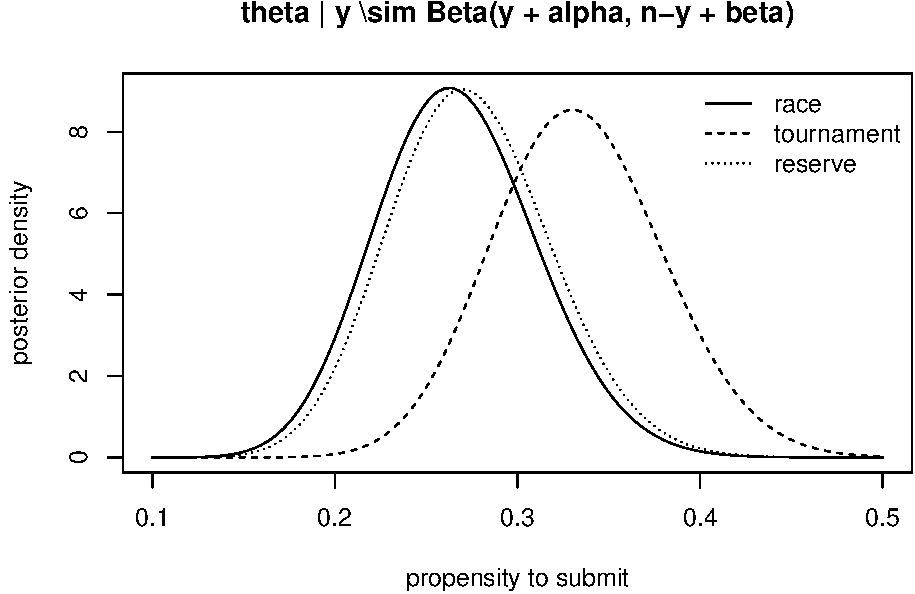
\includegraphics{Figures/unnamed-chunk-5-1.pdf}

\begin{table}
\centering
\caption{Outcomes by rooms}
\label{outcomes}
\begin{tabular}{@{}lm{2cm}m{2cm}m{2cm}m{2cm}}
  \\[-1.8ex]\hline\hline\\[-1.8ex]
 & Treatment & N & Participants & Submissions \\ 
  \hline\\[-1.86ex]
1 & Race & 9 & 2 & 80 \\ 
  2 & Race & 10 & 2 & 31 \\ 
  3 & Race & 10 & 5 & 95 \\ 
  4 & Race & 10 & 1 & 58 \\ 
  5 & Race & 15 & 4 & 178 \\ 
  6 & Race & 15 & 3 & 49 \\ 
  7 & Race & 15 & 4 & 31 \\ 
  8 & Race & 15 & 5 & 144 \\ 
  9 & Tournament & 10 & 3 & 39 \\ 
  10 & Tournament & 10 & 5 & 96 \\ 
  11 & Tournament & 10 & 5 & 33 \\ 
  12 & Tournament & 10 & 2 & 110 \\ 
  13 & Tournament & 15 & 5 & 242 \\ 
  14 & Tournament & 15 & 4 & 30 \\ 
  15 & Tournament & 15 & 4 & 15 \\ 
  16 & Tournament & 15 & 5 & 39 \\ 
  17 & Reserve & 10 & 1 & 2 \\ 
  18 & Reserve & 10 & 3 & 51 \\ 
  19 & Reserve & 10 & 3 & 64 \\ 
  20 & Reserve & 10 & 2 & 46 \\ 
  21 & Reserve & 15 & 4 & 25 \\ 
  22 & Reserve & 15 & 6 & 142 \\ 
  23 & Reserve & 15 & 3 & 67 \\ 
  24 & Reserve & 15 & 5 & 92 \\ 
   \hline\\[-1.8ex]
\end{tabular}
\end{table}

To understand xxxx, we now specify a logistic regression model for the
conditional probability of entry (\(Y_i=1\)) given the assignment
\((Z_i=1,2,3)\) and a matrix of control variables (\(X_i\)):

\begin{equation}
    \Pr(Y_i = 1 \mid X_i=x, Z_i=z) = \Lambda (xxxx...) 
\end{equation}

\begin{verbatim}
## 
##  Kruskal-Wallis rank sum test
## 
## data:  rating_l
## Kruskal-Wallis chi-squared = 2, df = 2, p-value = 0.4
\end{verbatim}

\begin{verbatim}
## 
##  Welch Two Sample t-test
## 
## data:  rating_l$Race and rating_l$Tournament
## t = -0.4, df = 50, p-value = 0.7
## alternative hypothesis: true difference in means is not equal to 0
## 95 percent confidence interval:
##  -331  218
## sample estimates:
## mean of x mean of y 
##      1452      1509
\end{verbatim}

\subsubsection{Room size}\label{room-size}

Our model also predicts lower participation for individuals in large
rooms (15 competitors) compared to those in small rooms (10
competitors). Under the model, the ``marginal type'' is increasing in
group size and so the individual probability of entry is lower. However,
our data proved only negligible differences in participation between
large (28.9 percent) and small rooms (28.6 percent). Additionally, we
found no significant treatment differences conditional on the room size
being large or small (xxxxx). Hence, one may conclude that a group-size
difference of 5 people is probably not large enough to be impactful.

\begin{verbatim}
## 
##  Welch Two Sample t-test
## 
## data:  nsub_l$race and nsub_l$tournament
## t = 0.6, df = 50, p-value = 0.5
## alternative hypothesis: true difference in means is not equal to 0
## 95 percent confidence interval:
##  -0.594  1.128
## sample estimates:
## mean of x mean of y 
##      2.20      1.93
\end{verbatim}

\begin{verbatim}
## 
##  Wilcoxon rank sum test with continuity correction
## 
## data:  nsub_l$race and nsub_l$tournament
## W = 500, p-value = 0.6
## alternative hypothesis: true location shift is not equal to 0
\end{verbatim}

The median submission per participant was of 0 submissions, with a
minimum of 0 and a maximum of 126 submissions.

\section{Participation by experience}\label{participation-by-experience}

\begin{verbatim}
## 
##  Pearson's Chi-squared test
## 
## data:  table(submit, mm_qtl)
## X-squared = 10, df = 3, p-value = 0.002
\end{verbatim}

\begin{verbatim}
##                   mm_qtl [1,3] (3,9] (9,25] (25,161]
## treatment  submit                                   
## Race       FALSE            25    15     16       17
##            TRUE              7     6      7        6
## Tournament FALSE            29    12     16       10
##            TRUE              7     5      6       15
## Reserve    FALSE            24    19     16       14
##            TRUE              1     6     10       10
\end{verbatim}

\begin{verbatim}
## 
## Call:
## glm(formula = submit ~ treatment + mm_qtl + hours_qtl, family = binomial)
## 
## Deviance Residuals: 
##    Min      1Q  Median      3Q     Max  
## -1.614  -0.816  -0.672   1.133   2.210  
## 
## Coefficients:
##                     Estimate Std. Error z value Pr(>|z|)    
## (Intercept)          -2.2115     0.4326   -5.11  3.2e-07 ***
## treatmentTournament   0.2918     0.3309    0.88   0.3780    
## treatmentReserve     -0.0597     0.3370   -0.18   0.8595    
## mm_qtl(3,9]           0.9197     0.4218    2.18   0.0292 *  
## mm_qtl(9,25]          1.1402     0.4018    2.84   0.0045 ** 
## mm_qtl(25,161]        1.7283     0.4005    4.32  1.6e-05 ***
## hours_qtl(16,24]      0.0721     0.3941    0.18   0.8547    
## hours_qtl(24,40]     -0.0802     0.3688   -0.22   0.8278    
## hours_qtl(40,192]     1.1760     0.3856    3.05   0.0023 ** 
## ---
## Signif. codes:  0 '***' 0.001 '**' 0.01 '*' 0.05 '.' 0.1 ' ' 1
## 
## (Dispersion parameter for binomial family taken to be 1)
## 
##     Null deviance: 358.81  on 298  degrees of freedom
## Residual deviance: 328.51  on 290  degrees of freedom
## AIC: 346.5
## 
## Number of Fisher Scoring iterations: 4
\end{verbatim}

\begin{verbatim}
## 
## Call:
## glm(formula = submit ~ treatment + mm_qtl + hours_qtl + mm_ratio, 
##     family = binomial)
## 
## Deviance Residuals: 
##    Min      1Q  Median      3Q     Max  
## -1.668  -0.810  -0.564   0.975   2.162  
## 
## Coefficients:
##                     Estimate Std. Error z value Pr(>|z|)    
## (Intercept)         -2.45557    0.45171   -5.44  5.4e-08 ***
## treatmentTournament  0.26603    0.33855    0.79  0.43198    
## treatmentReserve    -0.00304    0.34596   -0.01  0.99299    
## mm_qtl(3,9]          0.40630    0.45839    0.89  0.37543    
## mm_qtl(9,25]         0.56972    0.44021    1.29  0.19559    
## mm_qtl(25,161]       1.10642    0.44294    2.50  0.01249 *  
## hours_qtl(16,24]    -0.03374    0.40280   -0.08  0.93324    
## hours_qtl(24,40]    -0.04606    0.37609   -0.12  0.90252    
## hours_qtl(40,192]    1.14263    0.39488    2.89  0.00381 ** 
## mm_ratio             2.09779    0.63648    3.30  0.00098 ***
## ---
## Signif. codes:  0 '***' 0.001 '**' 0.01 '*' 0.05 '.' 0.1 ' ' 1
## 
## (Dispersion parameter for binomial family taken to be 1)
## 
##     Null deviance: 358.81  on 298  degrees of freedom
## Residual deviance: 317.30  on 289  degrees of freedom
## AIC: 337.3
## 
## Number of Fisher Scoring iterations: 4
\end{verbatim}

\begin{verbatim}
## Error in `contrasts<-`(`*tmp*`, value = contr.funs[1 + isOF[nn]]): contrasts can be applied only to factors with 2 or more levels
\end{verbatim}

\begin{verbatim}
## Error in `contrasts<-`(`*tmp*`, value = contr.funs[1 + isOF[nn]]): contrasts can be applied only to factors with 2 or more levels
\end{verbatim}

\begin{verbatim}
## Error in `contrasts<-`(`*tmp*`, value = contr.funs[1 + isOF[nn]]): contrasts can be applied only to factors with 2 or more levels
\end{verbatim}

\begin{verbatim}
## 
## ===============================================
##                         Dependent variable:    
##                     ---------------------------
##                               submit           
## -----------------------------------------------
## treatmentTournament            0.266           
##                               (0.339)          
##                                                
## treatmentReserve              -0.003           
##                               (0.346)          
##                                                
## mm_qtl(3,9]                    0.406           
##                               (0.458)          
##                                                
## mm_qtl(9,25]                   0.570           
##                               (0.440)          
##                                                
## mm_qtl(25,161]                1.110**          
##                               (0.443)          
##                                                
## hours_qtl(16,24]              -0.034           
##                               (0.403)          
##                                                
## hours_qtl(24,40]              -0.046           
##                               (0.376)          
##                                                
## hours_qtl(40,192]            1.140***          
##                               (0.395)          
##                                                
## mm_ratio                     2.100***          
##                               (0.636)          
##                                                
## Constant                     -2.460***         
##                               (0.452)          
##                                                
## -----------------------------------------------
## Observations                    299            
## Log Likelihood               -159.000          
## Akaike Inf. Crit.             337.000          
## ===============================================
## Note:               *p<0.1; **p<0.05; ***p<0.01
\end{verbatim}

\begin{verbatim}
##  setting  value                       
##  version  R version 3.3.2 (2016-10-31)
##  system   x86_64, darwin13.4.0        
##  ui       X11                         
##  language (EN)                        
##  collate  en_US.UTF-8                 
##  tz       America/New_York            
##  date     2017-06-20                  
## 
##  package   * version date       source        
##  backports   1.0.5   2017-01-18 CRAN (R 3.3.2)
##  boot      * 1.3-18  2016-02-23 CRAN (R 3.3.0)
##  devtools    1.12.0  2016-06-24 CRAN (R 3.3.0)
##  digest      0.6.12  2017-01-27 CRAN (R 3.3.2)
##  evaluate    0.10    2016-10-11 CRAN (R 3.3.0)
##  highr       0.6     2016-05-09 CRAN (R 3.3.0)
##  htmltools   0.3.5   2016-03-21 CRAN (R 3.3.0)
##  knitr       1.15.1  2016-11-22 CRAN (R 3.3.2)
##  lattice     0.20-34 2016-09-06 CRAN (R 3.3.2)
##  magrittr  * 1.5     2014-11-22 CRAN (R 3.3.0)
##  Matrix      1.2-7.1 2016-09-01 CRAN (R 3.3.2)
##  memoise     1.0.0   2016-01-29 CRAN (R 3.3.0)
##  races     * 0.2     2017-06-08 local (@0.2)  
##  Rcpp        0.12.9  2017-01-14 CRAN (R 3.3.2)
##  rmarkdown   1.3     2016-12-21 CRAN (R 3.3.2)
##  rprojroot   1.2     2017-01-16 CRAN (R 3.3.2)
##  stargazer * 5.2     2015-07-14 CRAN (R 3.3.0)
##  stringi     1.1.2   2016-10-01 CRAN (R 3.3.0)
##  stringr     1.2.0   2017-02-18 CRAN (R 3.3.2)
##  survival  * 2.40-1  2016-10-30 CRAN (R 3.3.0)
##  withr       1.0.2   2016-06-20 CRAN (R 3.3.0)
##  xtable    * 1.8-2   2016-02-05 CRAN (R 3.3.0)
##  yaml        2.1.14  2016-11-12 CRAN (R 3.3.2)
\end{verbatim}

\section*{References}\label{references}
\addcontentsline{toc}{section}{References}

\hypertarget{refs}{}
\hypertarget{ref-athey2002identification}{}
Athey, Susan, and Philip A Haile. 2002. ``Identification of Standard
Auction Models.'' \emph{Econometrica} 70 (6). Wiley Online Library:
2107--40.

\hypertarget{ref-athey2007nonparametric}{}
---------. 2007. ``Nonparametric Approaches to Auctions.''
\emph{Handbook of Econometrics} 6. Elsevier: 3847--3965.

\hypertarget{ref-athey2011comparing}{}
Athey, Susan, Jonathan Levin, and Enrique Seira. 2011. ``Comparing Open
and Sealed Bid Auctions: Evidence from Timber Auctions*.'' \emph{The
Quarterly Journal of Economics} 126 (1). Oxford University Press:
207--57.

\hypertarget{ref-baye2003strategic}{}
Baye, Michael R, and Heidrun C Hoppe. 2003. ``The Strategic Equivalence
of Rent-Seeking, Innovation, and Patent-Race Games.'' \emph{Games and
Economic Behavior} 44 (2). Elsevier: 217--26.

\hypertarget{ref-bimpikis2014designing}{}
Bimpikis, Kostas, Shayan Ehsani, and Mohamed Mostagir. 2014. ``Designing
Dynamic Contests.'' Working paper, Stanford University.

\hypertarget{ref-che2003optimal}{}
Che, Yeon-Koo, and Ian Gale. 2003. ``Optimal Design of Research
Contests.'' \emph{The American Economic Review} 93 (3). American
Economic Association: 646--71.

\hypertarget{ref-dechenaux2014survey}{}
Dechenaux, Emmanuel, Dan Kovenock, and Roman M Sheremeta. 2014. ``A
Survey of Experimental Research on Contests, All-Pay Auctions and
Tournaments.'' \emph{Experimental Economics}. Springer, 1--61.

\hypertarget{ref-dixit1987strategic}{}
Dixit, Avinash Kamalakar. 1987. ``Strategic Behavior in Contests.''
\emph{The American Economic Review} 77 (5). American Economic
Association: 891--98.

\hypertarget{ref-dohmen2011individual}{}
Dohmen, Thomas, Armin Falk, David Huffman, Uwe Sunde, Jürgen Schupp, and
Gert G Wagner. 2011. ``Individual Risk Attitudes: Measurement,
Determinants, and Behavioral Consequences.'' \emph{Journal of the
European Economic Association} 9 (3). Wiley Online Library: 522--50.

\hypertarget{ref-donald1996identification}{}
Donald, Stephen G, and Harry J Paarsch. 1996. ``Identification,
Estimation, and Testing in Parametric Empirical Models of Auctions
Within the Independent Private Values Paradigm.'' \emph{Econometric
Theory} 12 (03). Cambridge Univ Press: 517--67.

\hypertarget{ref-good2014microtask}{}
Good, Benjamin M, Max Nanis, CHUNLEI Wu, and ANDREW I Su. 2014.
``Microtask Crowdsourcing for Disease Mention Annotation in Pubmed
Abstracts.'' In \emph{Pacific Symposium on Biocomputing. Pacific
Symposium on Biocomputing}, 282--93. NIH Public Access.

\hypertarget{ref-green1983comparison}{}
Green, Jerry R, and Nancy L Stokey. 1983. ``A Comparison of Tournaments
and Contracts.'' \emph{The Journal of Political Economy} 91 (3):
349--64.

\hypertarget{ref-grossman1987dynamic}{}
Grossman, Gene M, and Carl Shapiro. 1987. ``Dynamic R\&D Competition.''
\emph{Economic Journal} 97 (386). Royal Economic Society: 372--87.

\hypertarget{ref-harris1987racing}{}
Harris, Christopher, and John Vickers. 1987. ``Racing with
Uncertainty.'' \emph{The Review of Economic Studies} 54 (1). Oxford
University Press: 1--21.

\hypertarget{ref-laffont1995econometrics}{}
Laffont, Jean-Jacques, Herve Ossard, and Quang Vuong. 1995.
``Econometrics of First-Price Auctions.'' \emph{Econometrica} 63 (4).
Econometric Society: 953--80.

\hypertarget{ref-lazear1981rank}{}
Lazear, Edward P, and Sherwin Rosen. 1981. ``Rank-Order Tournaments as
Optimum Labor Contracts.'' \emph{The Journal of Political Economy} 89
(5): 841--64.

\hypertarget{ref-leaman2008banner}{}
Leaman, Robert, Graciela Gonzalez, and others. 2008. ``BANNER: An
Executable Survey of Advances in Biomedical Named Entity Recognition.''
In \emph{Pacific Symposium on Biocomputing}, 13:652--63.

\hypertarget{ref-mary1984economic}{}
Mary, O'Keeffe, W Kip Viscusi, and Richard J Zeckhauser. 1984.
``Economic Contests: Comparative Reward Schemes.'' \emph{Journal of
Labor Economics} 2 (1). University of Chicago Press: 27--56.

\hypertarget{ref-moldovanu2001optimal}{}
Moldovanu, Benny, and Aner Sela. 2001. ``The Optimal Allocation of
Prizes in Contests.'' \emph{The American Economic Review}. JSTOR,
542--58.

\hypertarget{ref-moldovanu2006contest}{}
---------. 2006. ``Contest Architecture.'' \emph{Journal of Economic
Theory} 126 (1). Elsevier: 70--96.

\hypertarget{ref-paarsch1992deciding}{}
Paarsch, Harry J. 1992. ``Deciding Between the Common and Private Value
Paradigms in Empirical Models of Auctions.'' \emph{Journal of
Econometrics} 51 (1-2). Elsevier: 191--215.

\hypertarget{ref-parreiras2010contests}{}
Parreiras, Sérgio O, and Anna Rubinchik. 2010. ``Contests with Three or
More Heterogeneous Agents.'' \emph{Games and Economic Behavior} 68 (2).
Elsevier: 703--15.

\hypertarget{ref-siegel2009all}{}
Siegel, Ron. 2009. ``All-Pay Contests.'' \emph{Econometrica} 77 (1).
Wiley Online Library: 71--92.

\hypertarget{ref-siegel2014contests}{}
---------. 2014. ``Contests with Productive Effort.''
\emph{International Journal of Game Theory} 43 (3). Springer: 515--23.

\hypertarget{ref-szymanski2003economic}{}
Szymanski, Stefan. 2003. ``The Economic Design of Sporting Contests.''
\emph{Journal of Economic Literature} 41 (4). American Economic
Association: 1137--87.

\hypertarget{ref-taylor1995digging}{}
Taylor, Curtis R. 1995. ``Digging for Golden Carrots: An Analysis of
Research Tournaments.'' \emph{The American Economic Review} 85 (4).
American Economic Association: 872--90.

\hypertarget{ref-zizzo2002racing}{}
Zizzo, Daniel John. 2002. ``Racing with Uncertainty: A Patent Race
Experiment.'' \emph{International Journal of Industrial Organization} 20
(6). Elsevier: 877--902.

\end{document}